\section{Appendices}
%
\subsection{Decay schemes}
%
\begin{multicolfloat}
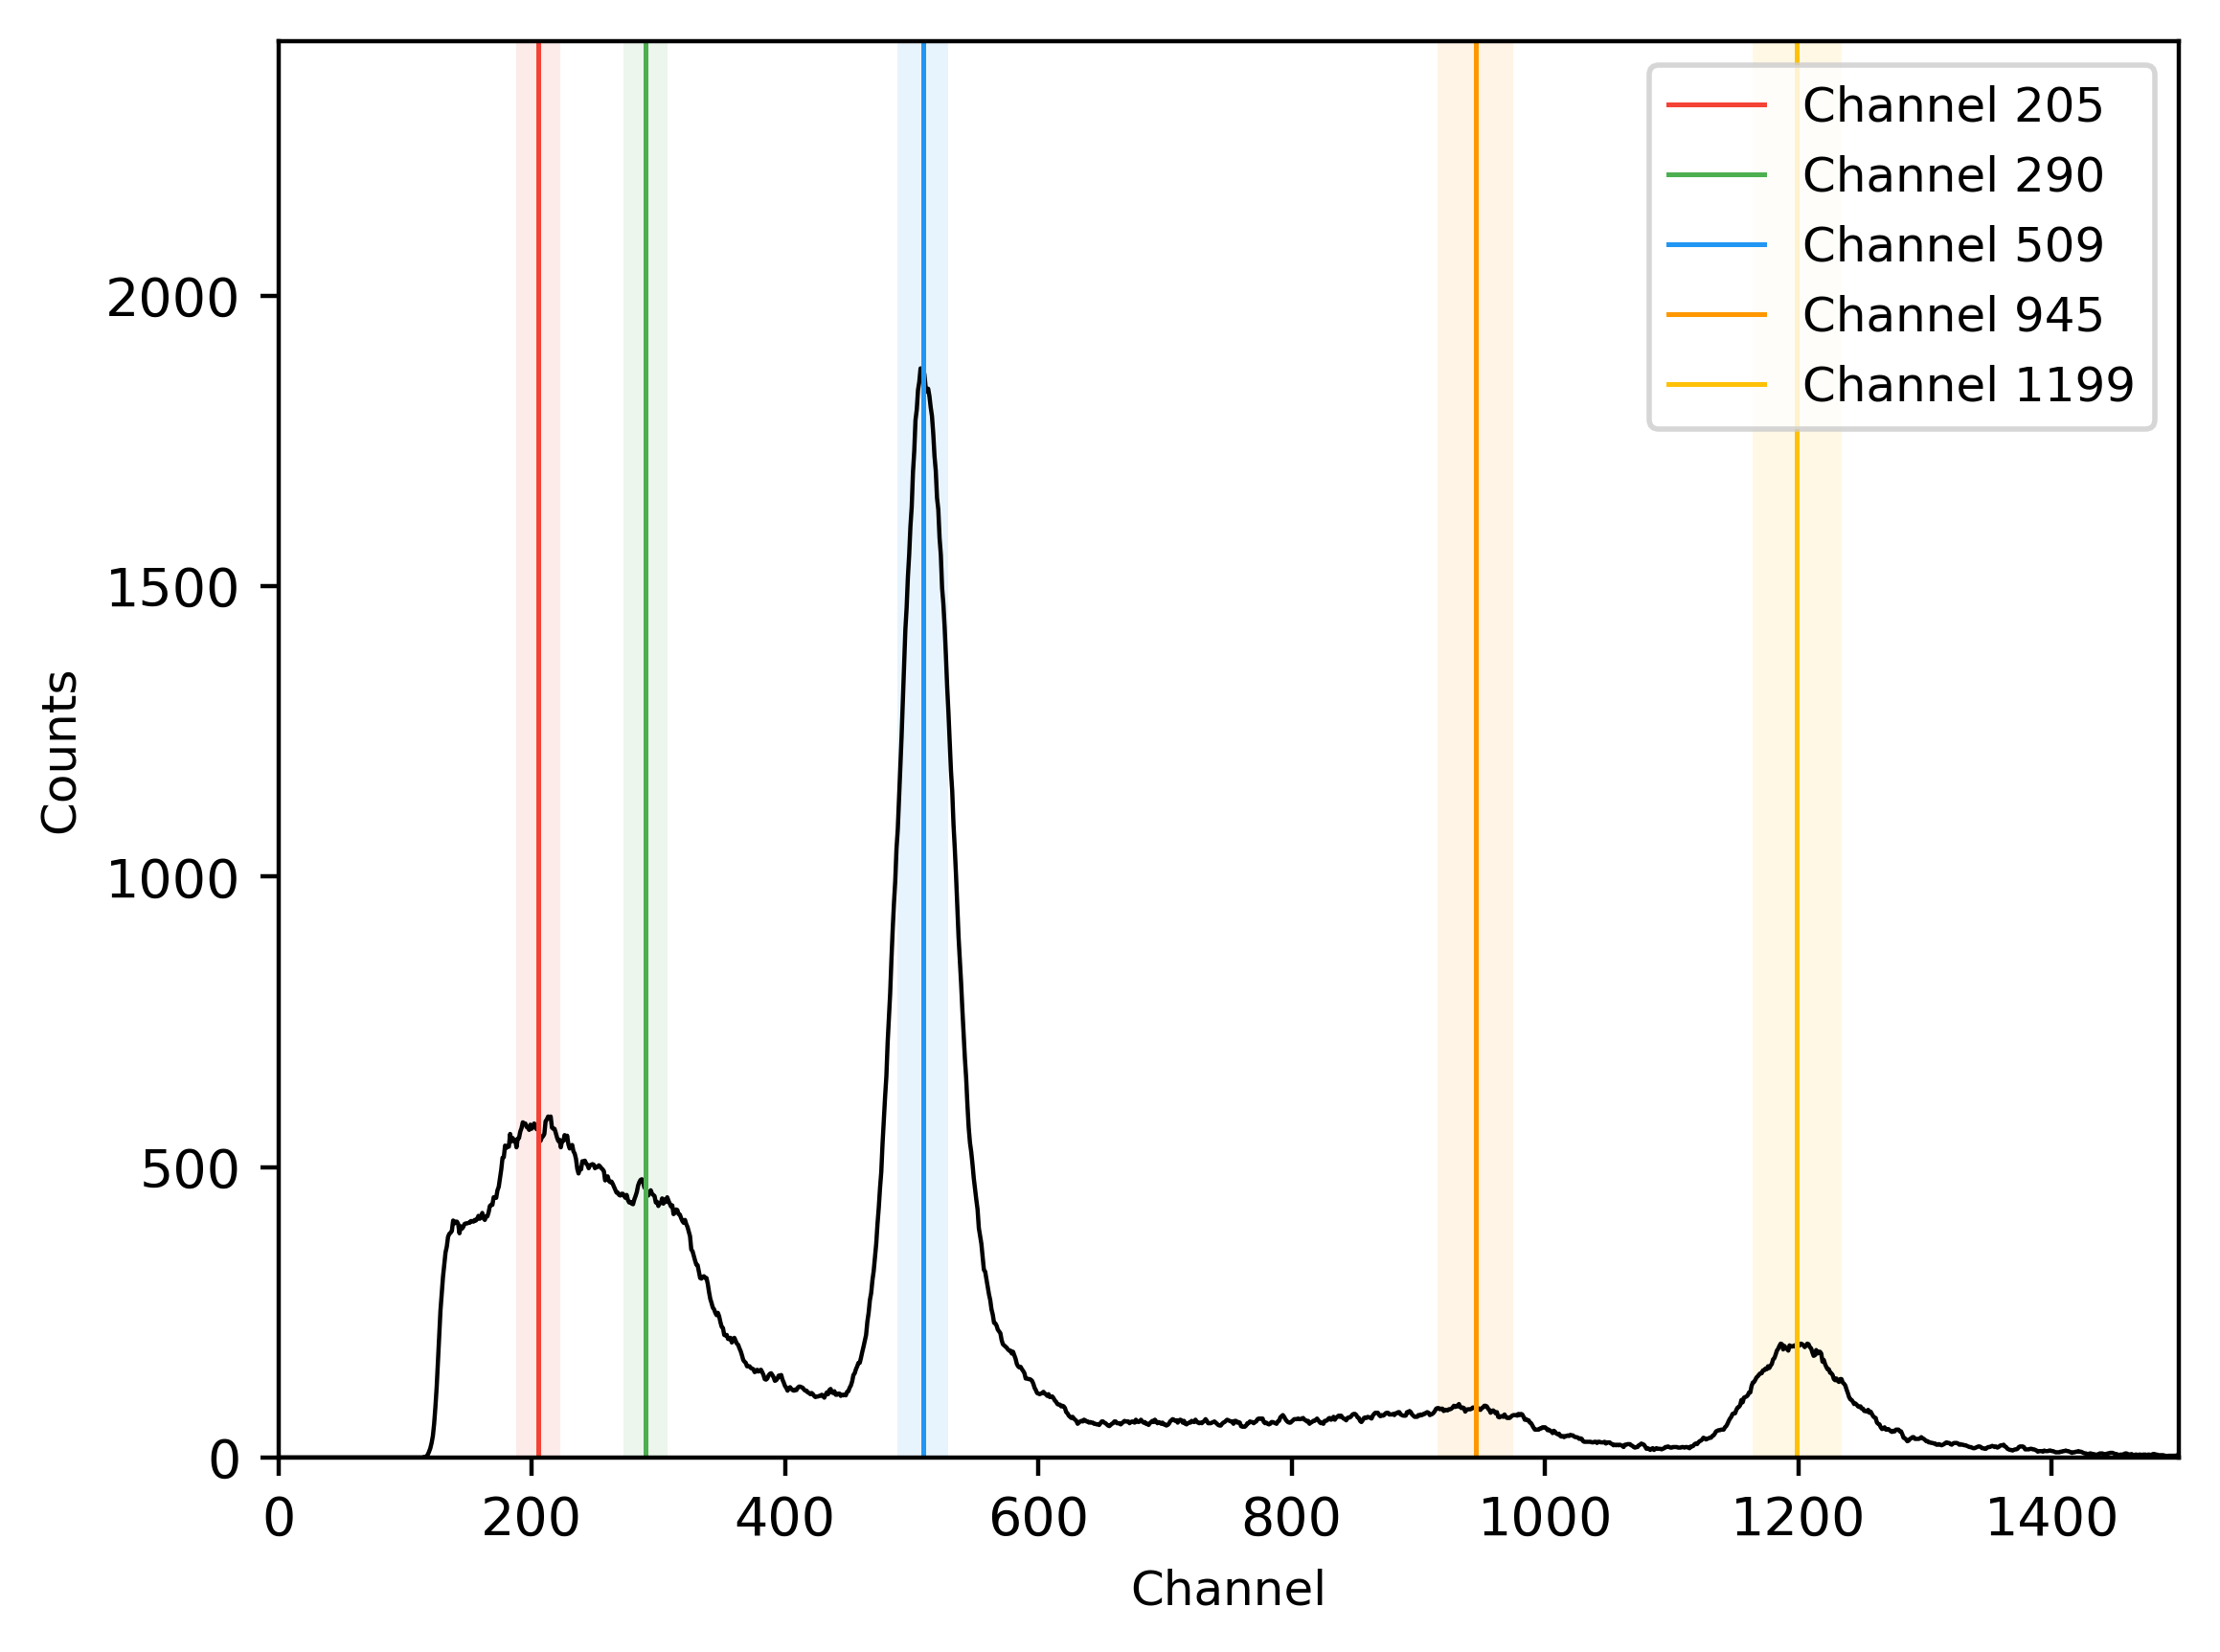
\includegraphics[width=\linewidth]{22Na}
\captionof{figure}{Decay scheme of $^{22}\text{Na}$}
\label{fig:22NaDecayScheme}
\end{multicolfloat}
%
\begin{multicolfloat}
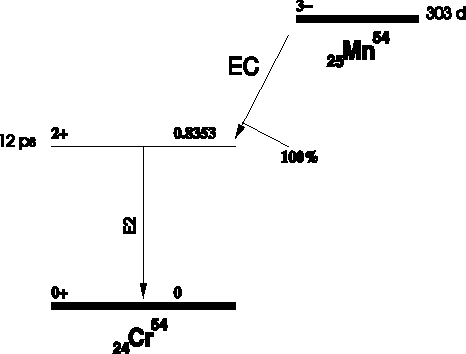
\includegraphics[width=\linewidth]{54Mn}
\captionof{figure}{Decay scheme of $^{54}\text{Mn}$}
\label{fig:54MnDecayScheme}
\end{multicolfloat}
%
\begin{multicolfloat}
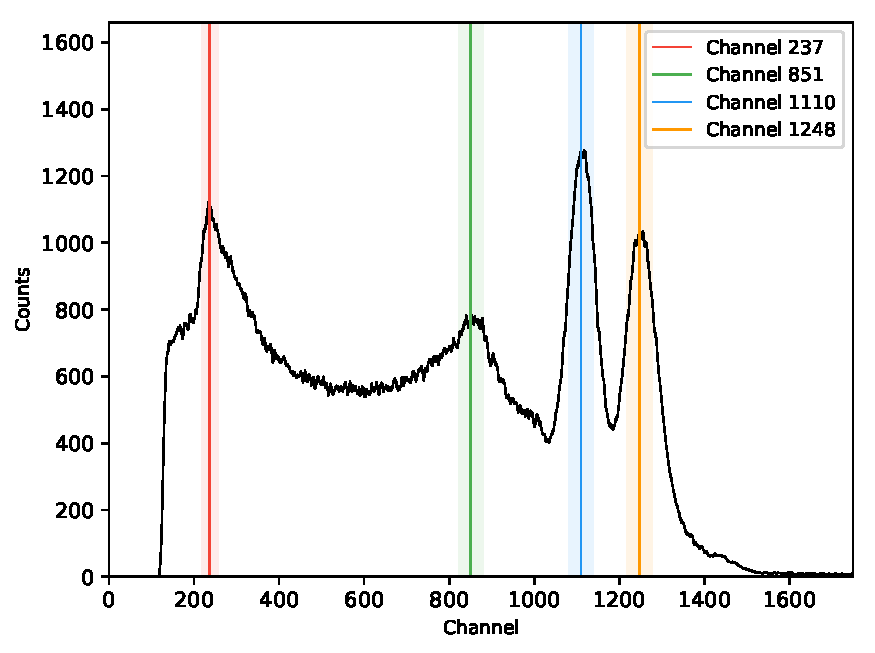
\includegraphics[width=\linewidth]{60Co}
\captionof{figure}{Decay scheme of $^{60}\text{Co}$}
\label{fig:60CoDecayScheme}
\end{multicolfloat}
%
\begin{multicolfloat}
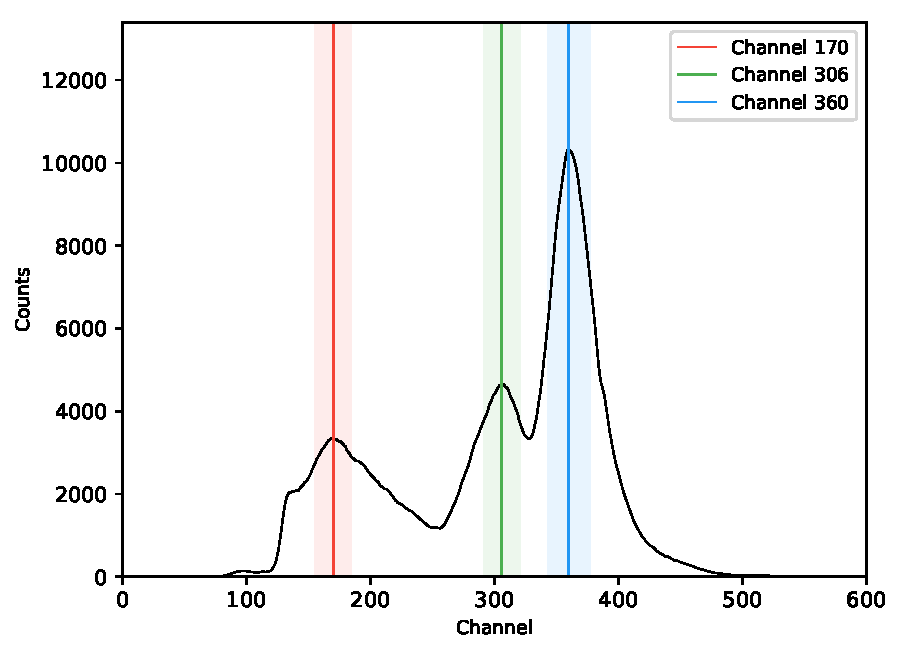
\includegraphics[width=\linewidth]{133Ba}
\captionof{figure}{Decay scheme of $^{133}\text{Ba}$}
\label{fig:133BaDecayScheme}
\end{multicolfloat}
%
\begin{multicolfloat}
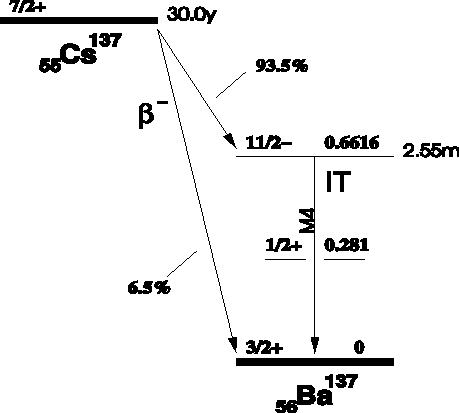
\includegraphics[width=\linewidth]{137Cs}
\captionof{figure}{Decay scheme of $^{137}\text{Cs}$}
\label{fig:137CsDecayScheme}
\end{multicolfloat}
%
\subsection{Circuit schematics}
%
\begin{multicolfloat}
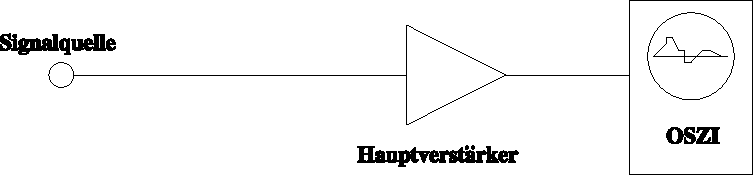
\includegraphics[width=\linewidth]{Schaltung1}
\captionof{figure}{Circuit schematic 1}
\label{fig:Schaltung1}
\end{multicolfloat}
%
\begin{multicolfloat}
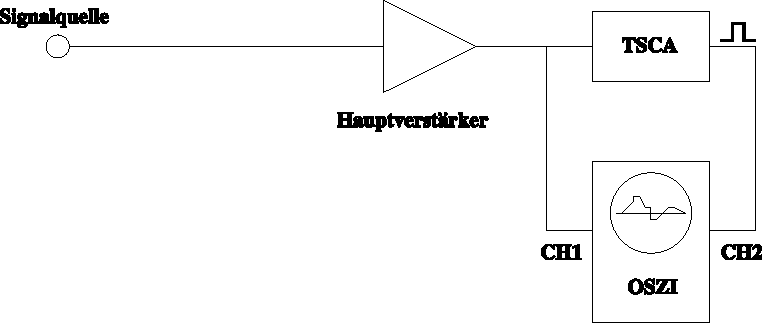
\includegraphics[width=\linewidth]{Schaltung2}
\captionof{figure}{Circuit schematic 2}
\label{fig:Schaltung2}
\end{multicolfloat}
%
\begin{multicolfloat}
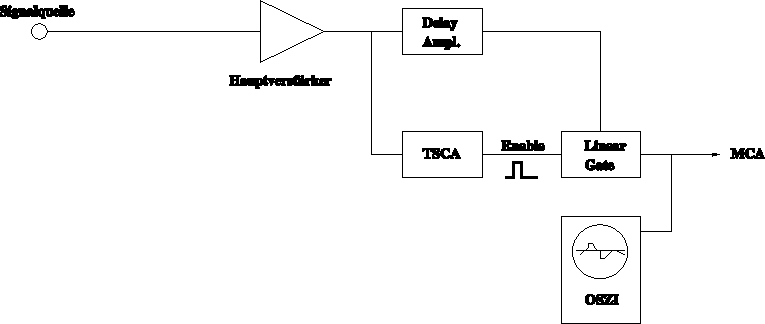
\includegraphics[width=\linewidth]{Schaltung3}
\captionof{figure}{Circuit schematic 3}
\label{fig:Schaltung3}
\end{multicolfloat}
%
\begin{multicolfloat}
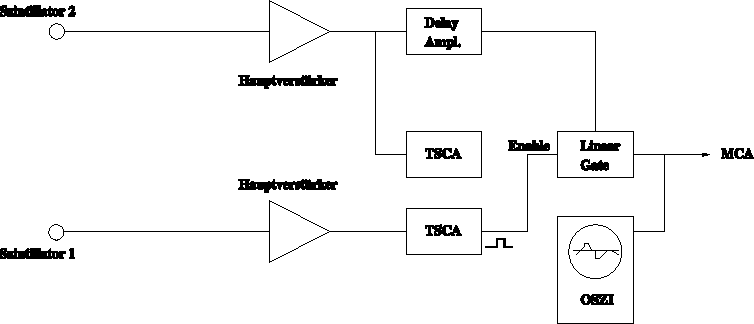
\includegraphics[width=\linewidth]{Schaltung4}
\captionof{figure}{Circuit schematic 4}
\label{fig:Schaltung4}
\end{multicolfloat}
%
\begin{multicolfloat}
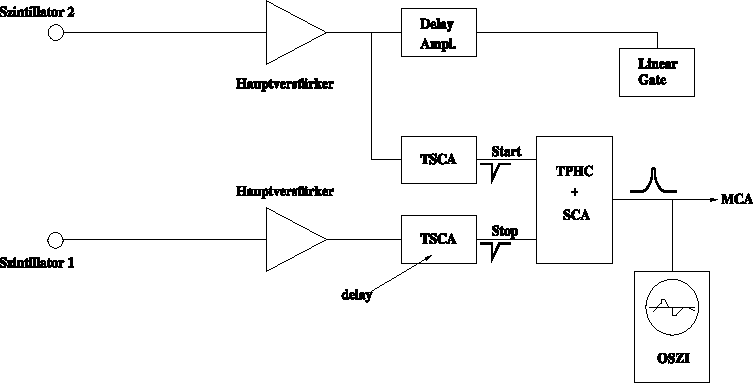
\includegraphics[width=\linewidth]{Schaltung5}
\captionof{figure}{Circuit schematic 5}
\label{fig:Schaltung5}
\end{multicolfloat}
%
\begin{multicolfloat}
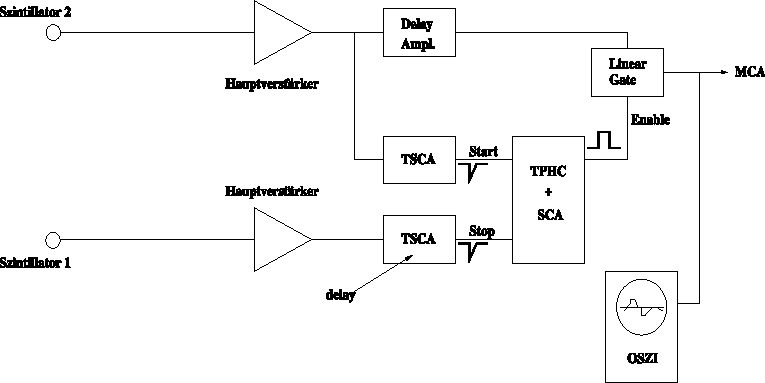
\includegraphics[width=\linewidth]{Schaltung6}
\captionof{figure}{Circuit schematic 6}
\label{fig:Schaltung6}
\end{multicolfloat}
